\documentclass[12pt]{article}
\usepackage[utf8]{inputenc}
\usepackage[T1]{fontenc}
\usepackage[german]{babel}
\usepackage{amsmath}
\usepackage{amsfonts}
\usepackage{amssymb}
\usepackage{lmodern}
\usepackage{graphicx}
\usepackage{enumerate}
\usepackage{stmaryrd}
\usepackage[dvipsnames,svgnames,x11names]{xcolor}
\usepackage[left=2cm,right=3.5cm,top=0cm,bottom=2cm,includeheadfoot]{geometry}
\usepackage[markup=underlined]{changes}

\setlength{\parindent}{0em}

\date{}

%--------------------------------

%Hier ist Platz für eigene Befehle. Einige sind schon vorgegeben.
\newcommand{\brackets}[1]{\left(#1\right)}
\newcommand{\setbr}[1]{\left\{#1\right\}}
\newcommand{\lpow}[1]{\!\left(\!\left(#1\right)\!\right)}
\newcommand{\pow}[1]{\!\left[\!\left[#1\right]\!\right]}
\newcommand{\norm}[1]{\left\|#1\right\|}
\newcommand{\abs}[1]{\left|#1\right|}
\newcommand{\sprod}[1]{\left<#1\right>}
\newcommand{\C}[0]{\mathbb{C}}
\newcommand{\R}[0]{\mathbb{R}}
\newcommand{\Q}[0]{\mathbb{Q}}
\newcommand{\Z}[0]{\mathbb{Z}}
\newcommand{\N}[0]{\mathbb{N}}
\newcommand{\F}[0]{\mathbb{F}}
\newcommand{\sphere}[0]{\mathbb{S}}
\renewcommand{\epsilon}[0]{\varepsilon}

\let\phi\varphi

\def\K{\mathbb{K}}

\DeclareMathOperator{\id}{id}

%--------------------------------

%Für Tutoren: Hier können weitere Kommentarfarben festgelegt werden und Kürzel festgelegt werden.
\definechangesauthor[color=BrickRed]{Fehler}
\definechangesauthor[color=NavyBlue]{Komm.}

\usepackage{todonotes}
\setcommentmarkup{\todo[color={authorcolor!20},size=\scriptsize]{#3: #1}}

\newcommand{\note}[2][]{\added[#1,comment={#2}]{}}
\newcommand{\richtig}[0]{{\color{red}\checkmark\  }}
\newcommand{\punkte}[1]{\hfill {\color{red} #1}}
\newcommand{\rot}[1]{{\color{red} #1}}
\newcommand{\ungenau}[0]{\note[id=Fehler]{Zu ungenau!}}
\newcommand{\gut}[0]{\note[id=Komm.]{Gut!}}
\newcommand{\sehrgut}[0]{\note[id=Komm.]{Sehr gut!}}
\newcommand{\kommentarkurz}[1]{\note[id=Komm.]{#1}}
\newcommand{\kommentarlang}[2]{\added[id=Komm.,comment={#2}]{#1}}
\newcommand{\fehlerkurz}[1]{\note[id=Fehler]{#1}}
\newcommand{\fehlerlang}[2]{\added[id=Fehler,comment={#2}]{#1}}
\newcommand{\einschub}[1]{\todo[inline, inlinewidth=5cm, noinlinepar]{#1}}
\title{Dokumentation "Das SIR-Modell in der mathematischen Epidemiologie"}
\author{Louisa Weber, Bernhard Eisvogel}

\begin{document}

	\maketitle

	
	\vspace{17cm}
	
	\small \vspace{-1mm} Computereinsatz in der Mathematik\hfill Universität Konstanz\\ Sommersemester~2020\hfill Fachbereich Mathematik und Statistik

\newpage
\tableofcontents
\newpage

\section{Infos}
Dies ist die zugehörige Dokumentation zum Abschlussprojekt "Das SIR-Modell in der mathematischen Epidemiologie" im Fach "Computereinsatz in der Mathematik" an der Universität Konstanz im Sommersemester 2020 von Louisa Weber und Bernhard Eisvogel. Es werden die Funktionen in den Programmdateien \verb|methods.py| und \verb|corona.py| dokumentiert sowie die auf dem Arbeitsblatt gestellten Fragen beantwortet. Außerdem werden die Zusatzaufgaben $1$ und $2$ behandelt. Am Ende werden wir uns der Frage widmen, welche Impfrate man gebraucht zur Abwendung der Coronapandemie ohne Lockdown benötigt hätte, wenn schon vier Wochen nach dem erstem Coronapatienten in Deutschland eine Impfungen gefunden worden wäre.

\section{Programmieraufgaben}
\subsection{Aufgabe 1}
Die Funktion \verb|ForwardEuler| in \verb|methods.py|  ist das Kernstück der Modellierung und approximiert Lösungen für Differentialgleichungen. Als Eingabewerte wird die erste Ableitung der zu approximierenden Funktion, die Schrittweite, ein Startwert und der zu approximierende Punkt angenommen. Die Funktion \verb|ForwardKutta4|   in \verb|methods.py|  übernimmt die gleiche Aufgabe, benutzt aber anstelle des Euler-Verfahrens ein vierstufiges Runge-Kutta-Verfahren, das genauer ist und wenig mehr Rechenzeit benötigt.
\subsection{Aufgabe 2}
Die Funktion \verb|SirLesen()| übernimmt die geforderte Funktion und liest die Datei \verb|sir.param| ein. Sie gibt eine Liste mit den Werten $\gamma,\beta_0,T,s_0,i_0$ in respektiver Reihenfolge zurück.
\subsection{Aufgabe 3}
\subsection{Aufgabe 4}
Die Methode \verb|PhasenportraitEp()| in \verb|corona.py| zeichnet ein Phasenportrait des epidemischen SIR - Modells.
\begin{center}
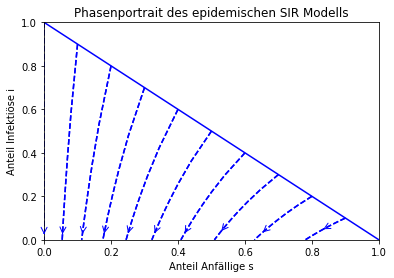
\includegraphics[scale=0.5]{PhasenportraitEpi.png}
\end{center}

\subsection{Aufgabe 5}
Die Funktion \verb|SirLesenDyn()| übernimmt die geforderte Funktion und liest die Datei \verb|sirdyn.param| ein. Sie gibt eine Liste mit den Werten $\gamma,\beta_0, \mu, T,s_0,i_0$ in respektiver Reihenfolge zurück.
\subsection{Aufgabe 6}
\subsection{Aufgabe 7}

\section{Zusatzaufgaben}

\subsection{Zusatzaufgabe 1}

\subsection{Zusatzaufgabe 2}


\section{Selbstgestellte Zusatzaufgaben}
\end{document}